\documentclass[12pt,a4paper,titlepage]{article}
\usepackage[utf8]{inputenc}
\usepackage{polski}
\usepackage{listings}
\usepackage{graphicx}
\usepackage{xcolor}
\usepackage{minted}
\makeatletter
\newcommand{\linia}{\rule{\linewidth}{0.4mm}}
\renewcommand{\maketitle}{\begin{titlepage}
    \vspace*{1cm}
    \begin{center}\small
    Politechnika Wrocławska\\
    Wydział Elektroniki\\
    Grafika Komputerowa i Komunikacja Człowiek-Komputer
    \end{center}
    \vspace{3cm}
    \noindent\linia
    \begin{center}
      \LARGE \textsc{\@title}
         \end{center}
     \linia
    \vspace{0.5cm}
    \begin{flushright}
    \begin{minipage}{7cm}
    \textit{\small Autor:}\\
    \normalsize \textsc{\@author} \par
    \end{minipage}
    \vspace{5cm}

     {\small czwartek, 17\textsuperscript{15}-20\textsuperscript{15} TN}\\
        mgr inż. Szymon Datko
     \end{flushright}
    \vspace*{\stretch{6}}
    \begin{center}
    \@date
    \end{center}
  \end{titlepage}%
}
\makeatother
\author{Justyna Skalska, 225942}
\title{Sprawozdanie nr 1\\
(Open GL - podstawy)}

\begin{document}

\maketitle
\section{Omówienie tematu}
Naszym zadaniem na pierwszych laboratoriach było stworzenie prostego programu przy użyciu biblioteki graficznej OpenGL wraz z rozszerzeniem GL Utility Toolkit (GLUT). Podczas ćwiczenia trzeba było wykonać kilka prostych zadań wprowadzających do wcześniej wspomnianej biblioteki. Polegały one na przekopiowaniu i przeanalizowaniu wklejonego kodu. Ostatnim zadaniem było narysowanie dywanu Sierpińskiego wraz z perturbacjami oraz kolorowaniem.

\section{Omówienie kodu}
Podczas zadania skorzystałam ze zdefiniowanego wcześniej typu \\ \mintinline{C++}{typedef float Point[2]}, który był tablicą dwóch elementów typu float. 

\begin{listing}[H]
\caption{Funkcja zwracająca losową liczbę}
\begin{minted}{C++}
float getRand() {
    return float(rand() % 1000) / 1000;
}
\end{minted}
\end{listing}

\begin{listing}[H]
\caption{Funkcja rysująca pojedynczy kwadrat}
\begin{minted}[linenos,breaklines]{C++}
void drawRectangle(Point a, Point b, Point c, Point d) {
    // zacznij rysowanie kształtu
    glBegin(GL_POLYGON);    
    // pobierz kolor pierwszego kąta
    glColor3f(getRand(), getRand(), getRand());
    // zdefiniuj pierwszy punkt kwadratu według współrzędnych
    glVertex2fv(a);
    glColor3f(getRand(), getRand(), getRand());
    glVertex2fv(b);
    glColor3f(getRand(), getRand(), getRand());
    glVertex2fv(c);
    glColor3f(getRand(), getRand(), getRand());
    glVertex2fv(d);
    // zakończ rysowanie kształtu
    glEnd();
}
\end{minted}
\end{listing}

\begin{listing}[H]
\caption{Funkcja rysująca dywan Sierpińskiego}
\begin{minted}[linenos,breaklines]{C++}
void drawSierpinskiCarpet(Point ld, Point rd, int level) {
    float width = (rd[0] - ld[0]) / 3;  // pobierz szerokość
    width += (getRand() * 2 - 1) / 5;   // generuj perturbacje
    
    float left, right;
    for (int i = 0; i < 3; i++) {
        for (int j = 0; j < 3; j++) {
            left = ld[0] + (width * i);
            right = ld[1] + (width * j);
            Point newLu = { left, right };  // nowy lewy górny punkt
            right += width;
            Point newLd = { left, right };  // nowy lewy dolny punkt
            left += width;
            Point newRu = { left, right };
            right -= width;
            Point newRd = { left, right };

            if ((i != 1) || (j != 1)) {
                if (level == 1)
                {
                    drawRectangle(newLu, newLd, newRu, newRd);
                } else {
                    drawSierpinskiCarpet(newLd, newRd, level - 1);
                }
            }
        }
    }
}
\end{minted}
\end{listing}

\begin{listing}[H]
\caption{Wywołanie funkcji rysowania dywanu Sierpińskiego}
\begin{minted}[linenos,breaklines]{C++}
// Funkcaja określająca, co ma być rysowane
// (zawsze wywoływana, gdy trzeba przerysować scenę)
void RenderScene(void) {
    glClear(GL_COLOR_BUFFER_BIT);
    
    // współrzędne skrajnych punktów dywanu
    Point ld = { -50, -50 };
    Point rd = { 50, -50 };

    int level = 3;  // stopień deformacji dywanu
    
    // wywołanie funkcji rysowania dywanu
    drawSierpinskiCarpet(ld, rd, level);     
    glFlush();
}
\end{minted}
\end{listing}
\newpage
\section{Rezultat prac}
Udało mi się wykonać wszystkie podpunkty zadania. Dzięki wykonanemu ćwiczeniu mogłam zapoznać się z podstawami działania oraz funkcjami biblioteki graficznej OpenGL.

\begin{figure}[H]
\centering
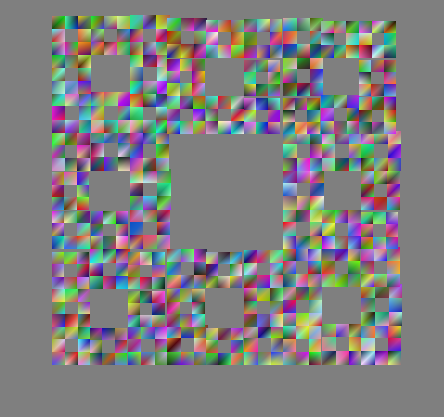
\includegraphics[width = 10cm]{sierpinskiCarpet.png}
\caption{Dywan Sierpińskiego z perturbacjami i kolorowaniem}
\label{fig:sierpinskiCarpet}
\end{figure}
\end{document}
